% !TeX root = main.tex

% TODO:
% - Replace `example' with `examples'
% - Use subsubsections

\documentclass[twoside]{report}

\usepackage[a4paper, margin=1in]{geometry}
\usepackage[utf8]{inputenc}
\usepackage{hyperref}
\usepackage{xcolor, textgreek, amssymb, amsmath, amsthm, tikz, graphicx, multirow, booktabs, bbold, listings, fancyhdr, titlecaps, cleveref}

\usetikzlibrary{automata, positioning, arrows, arrows.meta, calc, decorations.markings, circuits.logic.US}

\hypersetup{
    pdfauthor={Kit Matthewson},
    pdftitle={The Goblin Scrolls},
    pdfpagemode=FullScreen,
    colorlinks=true,
    linkcolor=black,
    filecolor=gray,
    urlcolor=teal,
    citecolor=black,
    breaklinks=false,
}

\newcounter{module}
\makeatletter
\@addtoreset{chapter}{part}
\makeatother
\newcommand{\module}[3]{%
    \setcounter{chapter}{0}%
    \setcounter{module}{#1}%
    \renewcommand{\partname}{Module}%
    \renewcommand{\thepart}{ECM\arabic{module}}%
    \part[#2]{#2\\\vspace{1\baselineskip}\small\emph{#3}}%
    \renewcommand{\partname}{Part}%
    \renewcommand{\thepart}{\Roman{part}}%
}

\newcommand{\tocchapter}[1]{%
  \stepcounter{chapter}%
  \addcontentsline{toc}{chapter}{\protect\numberline{\thechapter}#1}%
}

\newcommand{\tocsection}[1]{%
  \stepcounter{section}%
  \addcontentsline{toc}{section}{\protect\numberline{\thesection}#1}%
}

\renewcommand{\arraystretch}{1.2}

\renewcommand{\chaptermark}[1]{\markboth{#1}{}}

\definecolor{gruvbox-black}{HTML}{282828}
\definecolor{gruvbox-white}{HTML}{ebdbb2}
\definecolor{gruvbox-yellow}{HTML}{b57614}
\definecolor{gruvbox-purple}{HTML}{8f3f71}
\definecolor{gruvbox-blue}{HTML}{076678}
\definecolor{gruvbox-green}{HTML}{98971a}
\definecolor{gruvbox-red}{HTML}{cc241d}

\lstset{
    basicstyle=\color{gruvbox-black}\ttfamily,
    keywordstyle=\color{gruvbox-red},
    commentstyle=\color{gruvbox-blue},
    stringstyle=\color{gruvbox-green},
    numberstyle=\tiny\color{gruvbox-black},
    showspaces=false,
    showstringspaces=false,
    showtabs=false,
    columns=fullflexible,
    breaklines=true,
    postbreak=\mbox{\textcolor{gray}{\(\hookrightarrow\)}\space},
    escapechar=\$
}

\theoremstyle{definition}
\newtheorem{example}{Example}[section]
\newtheorem{examples}{Examples}[section]
\newtheorem{theorem}{Theorem}[section]

\newcommand*\parttitle{}
\let\origpart\part
\renewcommand*{\part}[2][]{%
    \ifx\\#1\\%
    \origpart{#2}%
        \renewcommand*\parttitle{#2}%
    \else
    \origpart[#1]{#2}%
        \renewcommand*\parttitle{#1}%
    \fi
}

\begin{document}

\renewcommand{\partname}{Module}
\renewcommand{\thepart}{ECM\arabic{part}}
\makeatletter
\@addtoreset{chapter}{part}
\makeatother
\newcommand{\module}[3]{%
    \setcounter{chapter}{0}%
    \setcounter{part}{#1}%
    \addtocounter{part}{-1}%
    \part[#2]{#2\\\vspace{1\baselineskip}\small\emph{#3}}
}

\renewcommand{\arraystretch}{1.2}

\renewcommand{\chaptermark}[1]{\markboth{#1}{}}

\definecolor{gruvbox-black}{HTML}{282828}
\definecolor{gruvbox-white}{HTML}{ebdbb2}
\definecolor{gruvbox-yellow}{HTML}{b57614}
\definecolor{gruvbox-purple}{HTML}{8f3f71}
\definecolor{gruvbox-blue}{HTML}{076678}
\definecolor{gruvbox-green}{HTML}{98971a}
\definecolor{gruvbox-red}{HTML}{cc241d}

\lstset{
    basicstyle=\color{gruvbox-black}\ttfamily,
    keywordstyle=\color{gruvbox-red},
    commentstyle=\color{gruvbox-blue},
    stringstyle=\color{gruvbox-green},
    numberstyle=\tiny\color{gruvbox-black},
    showspaces=false,
    showstringspaces=false,
    showtabs=false,
    columns=fullflexible,
    breaklines=true,
    postbreak=\mbox{\textcolor{gray}{\(\hookrightarrow\)}\space},
    escapechar=\$
}

\newcommand*\parttitle{}
\let\origpart\part
\renewcommand*{\part}[2][]{%
    \ifx\\#1\\%
    \origpart{#2}%
        \renewcommand*\parttitle{#2}%
    \else
    \origpart[#1]{#2}%
        \renewcommand*\parttitle{#1}%
    \fi
}


\begin{titlepage}

    \centering
    \vspace*{\baselineskip}

    \rule{\textwidth}{1.6pt}\vspace*{-\baselineskip}\vspace*{2pt}
    \rule{\textwidth}{0.4pt}

    \vspace{0.75\baselineskip}

    {\scshape\LARGE THE GOBLIN SCROLLS}

    \rule{\textwidth}{0.4pt}\vspace*{-\baselineskip}\vspace{3.2pt}
    \rule{\textwidth}{1.6pt}

    \vspace{2\baselineskip}

    Notes on the University of Exeter Computer Science course.

    \vspace*{5\baselineskip}

    Composed by the Sage of the Codes

    \vspace{0.5\baselineskip}

    {\scshape\Large Kit Matthewson}

    \vspace{1\baselineskip}

    As Unveiled to Him By

    \vspace{0.5\baselineskip}

    {\scshape\Large Jah}

    \vspace{10\baselineskip}

    Dedicated to

        {\scshape\normalsize His Imperial Majesty King Haile Selassie I\\Defender of the Faith,\\Reincarnation of the Son.}

    \vspace{12\baselineskip}

    As Declared on \today

\end{titlepage}

\tableofcontents

\clearpage

\pagestyle{fancy}
\fancyhead{}
\fancyhead[RE, LO]{The Goblin Scrolls}
\fancyhead[LE, RO]{\parttitle: \leftmark}
\fancyfoot{}
\fancyfoot[C]{\thepage}

\part{Notes}
\module{1011}{Fundamentals of Machine Learning}{Chico Camargo}

\chapter{Linear Regression}

% TODO Graphs

\section{Linear Regression}
Linear regression assumes one variable of a model is proportional to another:
\begin{equation}
    \label{eq:linear_regression}
    y = ax + b
\end{equation}
Non-linear regression, for instance quadratic, looks like:
\begin{equation*}
    y = ax^2 + bx + c
\end{equation*}
Or sigmoid:
\begin{equation*}
    y = \frac{1}{1 + e ^{b-x}}
\end{equation*}

\subsection{Fitting a regression model}
The values of \(a\) and \(b\) could be naively found by randomly sampling or using a grid search. A better method would iteratively search for the best values of \(a\) and \(b\). A generic parameter fitting method is:
\begin{lstlisting}
1. Start at a random point $\(\mathbf{P1}\)$ in parameter space.
2. Calculate the error at $\(\mathbf{P1}\)$.
3. Move to a nearby point $\(\mathbf{P2}\)$.
4. Calculate the error at $\(\mathbf{P2}\)$.
5. Stop when some condition is met.
\end{lstlisting}
A deterministic algorithm would calculate the position \(\mathbf{P2}\) to move to based on \(\mathbf{P1}\) and the calculated error. A stochastic algorithm picks a random point \(\mathbf{P2}\). A deterministic algorithm that uses some randomness will avoid getting `stuck' in local minima.

The conditions that need to be met for the algorithm to stop might include:
\begin{enumerate}
    \item The error going less than a certain threshold.
    \item Some number of steps having been taken.
\end{enumerate}

\subsection{Error functions}
Error can be calculated in two ways. L1 norm is:
\begin{equation*}
    \epsilon = \sum_{i=1}^{m}|y_i^{predicted} - y_i^{data}|
\end{equation*}
L2 norm replaces the modulus with a square, and is more common:
\begin{equation}
    \label{eq:l2_norm}
    \epsilon = \sqrt{\sum_{i=1}^{m}(y_i^{predicted} - y_i^{data})^2}
\end{equation}
The error function can also be called a cost or loss function. Note how \cref{eq:l2_norm} is also the formula for Euclidean distance.

\subsection{Deterministic fitting}
The deterministic algorithm needs to remember some information about the parameter space so that \(\mathbf{P2}\) can be determined. The best movement is to the minimum of the loss function, where the derivative of loss with respect to the parameters is 0:
\begin{align*}
    \frac{\delta loss}{\delta a} & = 0 \\
    \frac{\delta loss}{\delta b} & = 0
\end{align*}
Or:
\begin{equation*}
    \vec{\Delta} loss = 0
\end{equation*}
By finding the derivative of the loss function, the deterministic algorithm can move in the direction where the loss function has the steepest gradient.

\begin{lstlisting}
1. Start at a random point $\(\mathbf{P1}\)$ in parameter space.
2. Calculate the error at $\(\mathbf{P1}\)$.
3. Move in the direction of steepest gradient to point $\(\mathbf{P2}\)$.
4. Calculate the error at $\(\mathbf{P2}\)$.
5. Stop when the error has become less than a threshold, or more than $\(N\)$ steps have been taken.
\end{lstlisting}

\chapter{Classification Algorithms}

\section{Classification}
\subsection{Comparison to regression}
Classification tends to be used on discrete data, whereas regression is continuous. A classifier would be used to filter spam from email.

Adversarial data, like two objects that look similar to an image classifier, can `trick' a classification algorithm into producing an incorrect output.

A classifier will normally output a probability for each category that it knows. Any input given to the classifier will produce an output, even for inputs that do not actually fit into any category.

\subsection{Supervised learning}
Classification and regression are supervised learning techniques, because the algorithm is trained using correct examples, or `ground truth data'.

\subsection{Logistic regression}
Sigmoid regression (\cref{eq:sigmoid_regression}) could be used to fit a curve to data that fits into two categories, \(y=0\) and \(y=1\). In this case, the value of \(y\) is the probability that \(y=1\) for a given \(x\). This is called logistic regression.

\subsection{Cost functions}
L1 or L2 norm cannot be used on categorical algorithms because they rely on continuous data. Instead, the model is penalised based on how `obvious' the categorisation should be. For data in two categories, this looks like two exponentials that increase as the predicted probability of the correct category worsens.

\begin{table}[htbp]
    \centering
    \begin{tabular}{lll}
        \toprule
                           & Actual Positive & Actual Negative \\
        \midrule
        Predicted Positive & True Positive   & False Positive  \\
        Predicted Negative & False Positive  & True Negative   \\
        \bottomrule
    \end{tabular}
    \caption{Table Caption}
    \label{tab:label}
\end{table}

\section{Perceptrons}
\subsection{The Perceptron}
The perceptron mimics a biological neuron. A perceptron takes a list of inputs \(x_1 \dots x_k\) and parameters (or weights) \(w_1 \dots w_k\), and applies a function like a step function to their values to produce a single output from \(0\) to \(1\):
\begin{equation}
    \label{eq:perceptron_prediction}
    y^{pred} = f(\vec{w} \cdot \vec{x} + b)
\end{equation}
If the prediction \(y^{pred}\) is incorrect, the weights are updated with:
\begin{equation}
    \label{eq:perceptron_updating}
    \vec{w}_{t+1} = \vec{w}_t + \alpha(y^{data} - y^{pred})\vec{x}
\end{equation}
This can categorise data well only if it can be linear separated.

\subsection{Multi Layer Perceptron}
Many perceptrons can be connected together into a network. Multiple layers of perceptrons are connected so that the outputs of one layer become the inputs for the next. This leads to a large number of parameters that need to be fit. This is a neural network. A neural network with `lots' of layers is called a `deep neural network'.

Because of the large number of parameters, neural networks require a large amount of training data to produce accurate predictions.

\chapter{Probability}

\section{Probability distributions}
\subsection{Probabilities}
For a distribution with probability density function \(\mathrm{f}(x)\):
\begin{equation}
    \mathrm{P}(a < x < b) = \int_a^b \mathrm{f}(x)
\end{equation}

\subsection{Binning}
Binning a distribution refers to the process of taking a continuous distribution and turning it into a discrete distribution by creating discrete bin of values within ranges.

The bin sizes need to be chosen carefully so that key trends in the data are represented without showing meaningless noise in the data.

\subsection{Expected Value}
For a discrete distribution:
\begin{equation*}
    \mathrm{E}(X) = \mu_X = \sum x P(X = x)
\end{equation*}
For a continuous distribution:
\begin{equation*}
    \mathrm{E}(X) = \mu_X = \int x P(X = x) dx
\end{equation*}

\subsection{Variance and Standard Deviation}
For a discrete distribution:
\begin{equation}
    \mathrm{Var}(X) = \sigma_X^2 = \mathrm{E}(X^2) - \mathrm{E}(X)^2
\end{equation}
For a continuous distribution:
\begin{equation}
    \mathrm{Var}(X) = \sigma_X^2 = \mathrm{E}(X^2) - \mathrm{E}(X)^2
\end{equation}
Standard deviation is the square root of variance.

\subsection{Real data}
Real probability distributions can be described as:
\begin{itemize}
    \item Symmetric, or have skew to the left or right
    \item Uniform
    \item Unimodal, Bimodal, or Multimodal
\end{itemize}

\section{Common Distributions}
\subsection{Bell Distributions}
Bell shaped distributions include the binomial and normal. Most of the data is in the center. The shape is unimodal and symmetric with little skew.

\subsection{One-sided Distributions}
Ome-sided distributions have skew to one side, often because they are only valid for \(x > 0\). The Chi-squared, log normal, and Poisson are one-sided.

\subsection{Bernoulli Distributions}
A bernoulli distribution has two outcomes with probabilities \(p\) and \(1 - p\).

\section{Poisson Distributions}
\subsection{The Poisson distribution}
The Poisson distribution is notated as:
\begin{align*}
    X                 & \sim \mathrm{Po}(\lambda)          \\
    \mathrm{P}(X = x) & = \frac{e^{-\lambda}\lambda^x}{x!}
\end{align*}
Where \(\lambda\) is the mean rate.

\subsection{Modelling with the Poisson distribution}
The Poisson distribution is used to model the number of times \(X\) that a particular event occurs within a given interval. This could be an interval of any type, e.g. time or space.

In order for the Poisson distribution to be a good model, events must:
\begin{itemize}
    \item Be independent.
    \item Occur singly within their interval.
    \item Occur at a constant average rate.
\end{itemize}

\subsection{Adding Poisson distributions}
If \(X \sim \mathrm{Po}(\lambda)\) and \(Y \sim \mathrm{Po}(\mu)\):
\begin{equation*}
    X + Y \sim \mathrm{Po}(\lambda + \mu)
\end{equation*}

\subsection{Mean and Variance of a Poisson distribution}
If \(X \sim \mathrm{Po}(\lambda)\):
\begin{align*}
    \mathrm{E}(X)   & = \lambda \\
    \mathrm{Var}(X) & = \lambda
\end{align*}
The equivalence of the expected value and variance can be used to check that the Poisson is a suitable model.

\section{Exponential Distributions}
\subsection{The Exponential Distribution}
The exponential distribution has the density function:
\begin{equation*}
    P(X = x) = \lambda e^{-\lambda x} \{x \geq 0\}
\end{equation*}

\subsection{Mean and Variance of an Exponential distribution}
If \(X\) follows an exponential distribution:
\begin{align*}
    \mathrm{E}(X)   & = \frac{1}{\lambda}     \\
    \mathrm{Var}(X) & = \frac{1}{\lambda ^ 2}
\end{align*}

\section{Bayesian networks}
\subsection{Bayesian statistics}
For an event \(E\) that is dependent only on events \(A\) and \(B\), the probability \(\mathrm{P}(E)\) can be found with:
\begin{equation}
    \mathrm{P}(E) = \mathrm{P}(E | A) \times P(A) + \mathrm{P}(E | B) \times \mathrm{P}(B)
    \label{eq:dependent_probabilities}
\end{equation}

\subsection{Bayesian networks}
A chain of dependent events can be shown as a graph. The probability of any event in the graph depends only on its parents. The graph must be a directed acyclic graph (DAC).

This network is called a Bayesian network.

\begin{figure}[htbp]
    \centering
    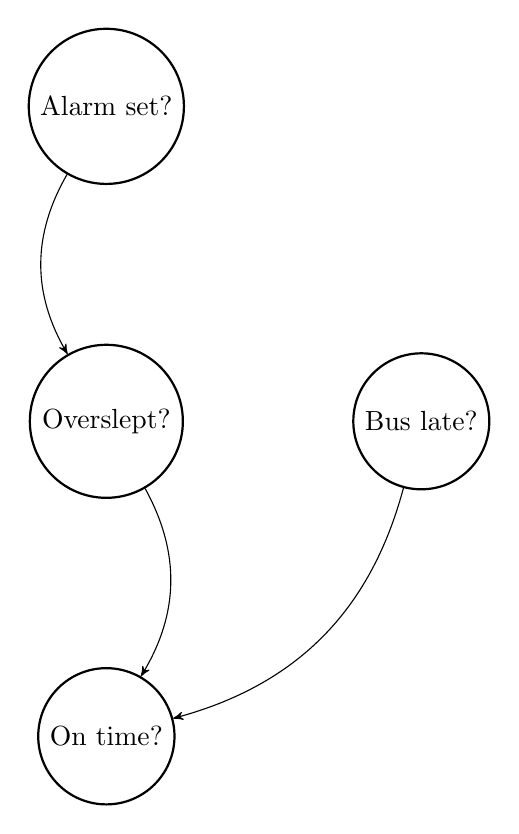
\begin{tikzpicture}
        \begin{scope}
            \tikzset{
                ->,
                >=stealth',
                node distance=4cm,
                every state/.style={thick},
                initial text=\( \),
            }

            \node[state] (alarm) {Alarm set?};
            \node[state, below of = alarm] (overslept) {Overslept?};
            \node[state, right of = overslept] (bus) {Bus late?};
            \node[state, below of = overslept] (ontime) {On time?};


            \draw (alarm) edge[bend right] (overslept);
            \draw (overslept) edge[bend left] (ontime);
            \draw (bus) edge[bend left] (ontime);

        \end{scope}
    \end{tikzpicture}
    \caption{Example Bayesian network where being on time depends on oversleeping and the bus being late, and oversleeping depends on the alarm being set.}
    \label{fig:bayesian_network}
\end{figure}

\subsection{Bayes' Theorem}
Rearranging \cref{eq:dependent_probabilities} gives Bayes' theorem:
\begin{equation}
    \mathrm{P}(A|B) = \frac{\mathrm{P}(B|A) \times \mathrm{P}(A)}{\mathrm{P}(B)}
    \label{eq:bayes_theorem}
\end{equation}
\begin{example}
    For a test for a disease, the equation would look like:
    \begin{equation*}
        \mathrm{P}(infected|\textit{tested positive}) = \frac{\mathrm{P}(\textit{tested positive}|infected) \times \mathrm{P}(infected)}{\mathrm{P}(\textit{tested positive})}
    \end{equation*}
\end{example}

\subsection{Application of Bayes' Theorem}
The sensitivity of a test is the probability of a true positive result (\(\mathrm{P}(T_+|B)\)). The specificity is the probability of a true negative result (\(\mathrm{P}(T_- | \neg B)\)).

If \(\mathrm{P}(B)\) is small, then \(\mathrm{P}(B|A)\) will also be small.

\section{Statistical Inference}
\subsection{Assumptions}
We start with a prior distribution that us updated with more data to generate a posterior distribution. This is the Bayesian approach, because priors are being used. The frequentist approach does not use priors.

There is no single estimate as output, instead a distribution of values.

\subsection{Maximum Likelihood Estimation}
From a sample of data \(x_1, x_2, \dots, x_n\), the best parameters for the distribution \(X\) are the ones that give the highest value of \(\mathrm{P}(x_1) \times \mathrm{P}(x_2) \times \dots \times \mathrm{P}(x_n)\).

For a normal distribution this means where:
\begin{align*}
    \frac{\delta P}{\delta \theta} & = 0 \\
    \frac{\delta P}{\delta \mu}    & = 0
\end{align*}
This gives a maximum likelihood estimate. The likelihood of the parameters taking certain values given some data is the probability of the model producing that data given those parameters: \(\mathrm{L}(\mu, \sigma | data) = \mathrm{P}(data | \mu, \sigma)\).
For a distribution with parameter \(\theta\) with data \(x\):
\begin{equation}
    \mathrm{P}(\theta | x) = \frac{\mathrm{P}(x | \theta)\mathrm{P}(\theta)}{\mathrm{P}(x)}
\end{equation}
The denominator acts as a normalising factor so that all probabilities sum to \(1\). The statement `find \(\theta\) such that \(\mathrm{P}(\theta|x)\) has its maximum value' is denoted:
\begin{equation*}
    \hat{\theta} = \arg \max_\theta \mathrm{P}(\theta|x)
\end{equation*}


\module{1400}{Programming}{Matt Collison}

\chapter{Introduction}

\section{Python}
Python is an interpreted, dynamically-typed programming language.

\section{Definitions}
An algorithm is a set of well defined instructions.

Programming languages are formal languages for instructing a computer.

A program is a set of instructions written in a programming language.

\chapter{Python basics}

\begin{lstlisting}[language=Python, numbers=left]
x = 5  # Assign the value 5 to the variable x
y = 10  # Assign the value 10 to the variable y

# If, Elif, Else
if x > y:
    print("x is greater than y")
elif x < y:
    print("x is less than y")
else:
    print("x is equal to y")

# For loop
for i in range(1, 6):
    print(i) # Prints 1, 2, 3, 4, 5

# While loop
counter = 0
while counter < 5:
    print(counter) # Prints 1, 2, 3, 4, 5
    counter += 1
\end{lstlisting}


\module{1407}{Social and Professional Issues of the Information Age}{Marcos Oliveira}

\module{1415}{Discrete Maths}{Diego Marmsoler}

\chapter{Logic and Proof}

\section{Propositional Logic}

\subsection{Propositions}
A proposition is a declarative sentence that is either true or false, for example:
\begin{itemize}
    \item The moon is made of green cheese.
    \item \(1 + 0 = 0\)
    \item \(0 + 0 = 2\)
\end{itemize}
Statements that are not proposition include:
\begin{itemize}
    \item ``Sit down"
    \item \(x + 1 = 2\)
\end{itemize}

\subsection{Propositional Logic}
Atomic propositions use variables (\(p\), \(q\), \(r\), \dots) and constants (\(\mathbf{T}\) and \(\mathbf{F}\)). Compound propositions use logic operators.

\subsubsection{Negation}
The negation (`not') of a proposition \(p\) is given by \(\neg p\). \(\neg p\) is true if \(p\) is false.

\begin{table}[htbp]
    \centering
    \begin{tabular}{cc}
        \toprule
        \(p\)          & \(\neg p\)     \\
        \midrule
        \(\mathbf{T}\) & \(\mathbf{F}\) \\
        \(\mathbf{F}\) & \(\mathbf{T}\) \\
        \bottomrule
    \end{tabular}
    \caption{Negation Truth Table}
\end{table}

\subsubsection{Conjunction}
The conjunction (`and') of propositions \(p\) and \(q\) is denoted by \(p \land q\). \(p \land q\) is true only if both \(p\) and \(q\) are true.

\begin{table}[htbp]
    \centering
    \begin{tabular}{ccc}
        \toprule
        \(p\)          & \(q\)          & \(p \land q\)  \\
        \midrule
        \(\mathbf{F}\) & \(\mathbf{F}\) & \(\mathbf{F}\) \\
        \(\mathbf{F}\) & \(\mathbf{T}\) & \(\mathbf{F}\) \\
        \(\mathbf{T}\) & \(\mathbf{F}\) & \(\mathbf{F}\) \\
        \(\mathbf{T}\) & \(\mathbf{T}\) & \(\mathbf{T}\) \\
        \bottomrule
    \end{tabular}
    \caption{Conjunction Truth Table}
\end{table}

\subsubsection{Disjunction}
The conjunction (`or') of propositions \(p\) and \(q\) is denoted by \(p \lor q\). \(p \lor q\) is true as long as at least one of \(p\) or \(q\) are true.

\begin{table}[htbp]
    \centering
    \begin{tabular}{ccc}
        \toprule
        \(p\)          & \(q\)          & \(p \lor q\)   \\
        \midrule
        \(\mathbf{F}\) & \(\mathbf{F}\) & \(\mathbf{F}\) \\
        \(\mathbf{F}\) & \(\mathbf{T}\) & \(\mathbf{T}\) \\
        \(\mathbf{T}\) & \(\mathbf{F}\) & \(\mathbf{T}\) \\
        \(\mathbf{T}\) & \(\mathbf{T}\) & \(\mathbf{T}\) \\
        \bottomrule
    \end{tabular}
    \caption{Disjunction Truth Table}
\end{table}

\subsubsection{Exclusive Or}
The exclusive or of propositions \(p\) and \(q\) is denoted by \(p \oplus q\). \(p \oplus q\) is true if \(p\) is true or \(q\) is true, but not both.

\begin{table}[htbp]
    \centering
    \begin{tabular}{ccc}
        \toprule
        \(p\)          & \(q\)          & \(p \oplus q\) \\
        \midrule
        \(\mathbf{F}\) & \(\mathbf{F}\) & \(\mathbf{F}\) \\
        \(\mathbf{F}\) & \(\mathbf{T}\) & \(\mathbf{T}\) \\
        \(\mathbf{T}\) & \(\mathbf{F}\) & \(\mathbf{T}\) \\
        \(\mathbf{T}\) & \(\mathbf{T}\) & \(\mathbf{F}\) \\
        \bottomrule
    \end{tabular}
    \caption{Exclusive Or Truth Table}
\end{table}

\subsection{Compound propositions}
If \(p\) and \(q\) are propositions, then \(p \rightarrow q\) is a conditional statement or implication. \(p\) is the hypothesis (or antecedent or premise), and \(q\) is the conclusion (or consequence).

\begin{table}[htbp]
    \centering
    \begin{tabular}{ccc}
        \toprule
        \(p\)          & \(q\)          & \(p \rightarrow q\) \\
        \midrule
        \(\mathbf{F}\) & \(\mathbf{F}\) & \(\mathbf{T}\)      \\
        \(\mathbf{F}\) & \(\mathbf{T}\) & \(\mathbf{T}\)      \\
        \(\mathbf{T}\) & \(\mathbf{F}\) & \(\mathbf{F}\)      \\
        \(\mathbf{T}\) & \(\mathbf{T}\) & \(\mathbf{T}\)      \\
        \bottomrule
    \end{tabular}
    \caption{Implication Truth Table}
\end{table}

Note how if the hypothesis is false, the implication always holds.

If \(p \rightarrow q\), `If it is raining I stay at home':
\begin{itemize}
    \item \(q \rightarrow p\) is the converse: `If I stay at home it is raining'.
    \item \(\neg q \rightarrow \neg p\) is the contrapositive: `If it is not raining I will not stay at home'.
    \item \(\neg p \rightarrow \neg q\) is the inverse: 'If I do not stay at home it is not raining.'.
\end{itemize}
If \(p\) and \(q\) are propositions, \(p \leftrightarrow  q\) is the biconditional `if and only if'.

\begin{table}[htbp]
    \centering
    \begin{tabular}{ccc}
        \toprule
        \(p\)          & \(q\)          & \(p \leftrightarrow q\) \\
        \midrule
        \(\mathbf{F}\) & \(\mathbf{F}\) & \(\mathbf{T}\)          \\
        \(\mathbf{F}\) & \(\mathbf{T}\) & \(\mathbf{F}\)          \\
        \(\mathbf{T}\) & \(\mathbf{F}\) & \(\mathbf{F}\)          \\
        \(\mathbf{T}\) & \(\mathbf{T}\) & \(\mathbf{T}\)          \\
        \bottomrule
    \end{tabular}
    \caption{Biconditional Truth Table}
\end{table}

A truth table can be constructed for compound propositions by creating a row for every combination of values for the atomic propositions, and a column for the truth value of every sub-expression.

A proposition that is always true, like \(p \lor \neg p\), is called a tautology. A contradiction like \(p \land \neg p\) is always false. A statement that can be either is a contingency.

The logical operators have the precedence:
\begin{enumerate}
    \item Negation \(\neg\)
    \item Conjunction \(\land\)
    \item Disjunction \(\lor\)
    \item Implication \(\rightarrow\)
    \item Biconditional \(\leftrightarrow\)
\end{enumerate}

\section{Propositional equivalences}

\subsection{Equivalence}
Two propositions \(p\) and \(q\) are equivalent if they have the same truth tables, shown by \(p \equiv q\). This is the same as saying that \(p \leftrightarrow q\) is a tautology.

The contrapositive of an implication is equivalent to the implication, but the inverse and converse are not.

\subsection{Key logical equivalences}
The identity law says that true is the identity of conjunction, and false the identity of disjunction:
\begin{align}
    p \land \mathbf{T} & \equiv p \\
    p \lor \mathbf{F}  & \equiv p
\end{align}
The domination law says that true dominates disjunction, and false dominates conjunction:
\begin{align}
    p \land \mathbf{F} & \equiv \mathbf{F} \\
    p \lor \mathbf{T}  & \equiv \mathbf{T}
\end{align}
The idempotent law says that the conjunction or disjunction of \(p\) with itself is \(p\):
\begin{align}
    p \land p & \equiv p \\
    p \lor p  & \equiv p
\end{align}
The double negative law says that two negatives do not change a variable:
\begin{align}
    \neg(\neg p) & \equiv p
\end{align}
The negation law says that the disjunction of \(p\) with \(\neg p\) is true, and the conjunction is false:
\begin{align}
    p \land \neg p & \equiv \mathbf{F} \\
    p \lor \neg p  & \equiv \mathbf{T}
\end{align}
The commutative law says that disjunction and conjunction are commutative:
\begin{align}
    p \land q & \equiv q \land p \\
    p \lor q  & \equiv q \lor p
\end{align}
The associative law says that the order that three conjunctions or disjunctions are evaluated does not matter:
\begin{align}
    p \land (q \land r) & \equiv (p \land q) \land r \\
    p \lor (q \lor r)   & \equiv (p \lor q) \lor r
\end{align}
The distributive law says that a disjunction or conjunction can be distributed across the other operator:
\begin{align}
    p \land (q \lor r) & \equiv p \land q \lor p \land r    \\
    p \lor (q \land r) & \equiv (p \lor q) \land (p \lor r)
\end{align}
The absorption law says that:
\begin{align}
    p \lor (p \land q) & \equiv p \\
    p \land (p \lor q) & \equiv p
\end{align}
De Morgan's laws state:
\begin{align}
    \neg(p \land q) & \equiv \neg p \lor \neg q  \\
    \neg(p \lor q)  & \equiv \neg p \land \neg q
\end{align}
Laws for conditional statements are:
\begin{align}
    p \rightarrow q & \equiv \neg p \lor q             \\
    p \rightarrow q & \equiv \neg q \rightarrow \neg p
\end{align}
And for biconditional statements:
\begin{align}
    p \leftrightarrow q & \equiv (p \rightarrow q) \lor (q \rightarrow p)
\end{align}

\subsection{Constructing new logical equivalences}
To prove that \(A \equiv B\), produce a series of equivalences that begins with \(A\) and ends with \(B\).

\chapter{Predicate Logic and Proof}

\section{Predicates and Quantifiers}
\subsection{Predicate Logic}
A predicate is a proposition that contains variables. Variables denote subjects with \(x\), \(y\), and \(z\). Predicates denote a property of a subject: \(P(x)\), \(M(x)\). Quantifiers quantify over subjects, for example \(\forall x\) and \(\exists x\).

\begin{example}
    Let \(P(x)\) denote \(x > 0\), then:
    \begin{itemize}
        \item \(P(3) \lor P(-1)\) is true
        \item \(P(3) \land P(-1)\) is false
        \item \(P(3 \land P(y))\) is not a proposition
    \end{itemize}
\end{example}
Predicates with multiple variables are denoted \(Q(x, y)\).

\subsection{Quantifiers}
The universal quantifier \(\forall\) means `for all'. \(\forall x. P(x)\) asserts that \(P(x)\) is true for every \(x\) in the domain. The existential quantifier \(\exists\) means `there exists'. \(\exists x. P(x)\) asserts that \(P(x)\) is true for some \(x\) in the domain\footnote{\(\exists!\) is sometimes used to denote `there exists exactly one'.}. Quantifiers have higher precedence than all logical quantifiers.

The domain is often denoted by \(U\), for universe of discourse.

\begin{example}
    If \(P(x)\) denotes `\(x\) is even', and \(U\) is the integers, then:
    \begin{itemize}
        \item \(\forall x. P(x)\) is false
        \item \(\exists x. P(x)\) is true
    \end{itemize}
\end{example}
The truth values of a predicate with a domain depends on both the domain and the predicate.

Quantifiers can be nested, so that a predicate with multiple quantifiers can be written. The statement `for every \(x\), there is a \(y\)\dots' is denoted \(\forall x \exists y. \dots\). The order of the quantifiers is important. For a proposition with the nested quantifiers \(\exists y \forall x\) to be true, the predicate must hold for some values of \(y\), no matter the value of \(x\).

\subsection{Equivalence}
Two statements involving predicates and quantifiers are logically equivalent if and only if they have the same truth value for every predicate substituted into these statements and for every domain used for the variables in the expressions.

De Morgan's laws for quantifiers are:
\begin{align*}
    \neg(\forall x. P(x)) & \equiv \exists x. \neg P(x) \\
    \neg(\exists x. P(x)) & \equiv \forall x. \neg P(x)
\end{align*}

\section{Rules of inference}
\subsection{Arguments}
An argument is a sequence of propositions.
\begin{itemize}
    \item All but the final proposition are called premises.
    \item The last statement is the conclusion.
    \item THe argument is valid if the premises imply the conclusion.
    \item An argument form is an argument that is valid no matter what propositions are substituted into its propositional variables.
\end{itemize}

\begin{example}
    An argument:
    \begin{equation*}
        \begin{array}{r l}
                       & Snowing \rightarrow Study \\
                       & Snowing                   \\
            \cline{2-2}
            \therefore & Study
        \end{array}
    \end{equation*}
    In argument form:
    \begin{equation*}
        \begin{array}{r l}
                       & p \rightarrow q \\
                       & p               \\
            \cline{2-2}
            \therefore & q
        \end{array}
    \end{equation*}
    The corresponding tautology is:
    \begin{equation*}
        (p \land (p \rightarrow q)) \rightarrow q
    \end{equation*}
\end{example}

\chapter{Set Theory}
\section{Sets}
\subsection{Basic Notation}
A set is an unordered collection of objects. The objects in a set are called its elements or members. A set is said to contain all its elements. The notation \(a \in A\) denotes that \(a\) is in set \(A\), \(a \notin A\) denotes that it is not.

The rooster method of denoting a set is \(S = \{a, b, c, d\}\). Ellipses can be used when a pattern is clear: \(S = \{a, b, c, \dots, \}\).

\begin{example}
    Sets include:
    \begin{itemize}
        \item Vowels in the english alphabet: \(V = \{a, e, i, o, u\}\).
        \item Integers less than \(0\): \(O = \{..., -3, -2, -1\}\).
    \end{itemize}
\end{example}
Set-builder notation specifies the properties that all members must satisfy.
\begin{example}
    \begin{equation*}
        S = {x | x \text{ is a positive integer less than } 100}
    \end{equation*}
    \begin{align*}
        [a, b] & = \{x | a \leq x \leq b\} \\
        (a, b) & =\{x | a < x < b\}        \\
        [a, b) & =\{x | a \leq x < b\}
    \end{align*}
\end{example}
Some important sets are:
\begin{align*}
    \mathbb{N}      & = \{0, 1, 2, 3, \dots\}                                                       \\
    \mathbb{Z}      & = \{\dots, -1, 0, 1, \dots\}                                                  \\
    \mathbb{Z^+}    & = \{1, 2, 3, \dots\}                                                          \\
    \mathbb{Q}      & = \{\frac{q}{p} | p \in \mathbf{Z}, q \in \mathbf{Z}, \text{ and } q \ne 0 \} \\
    \mathbb{R}      & = \text{all real numbers}                                                     \\
    \mathbf{U}      & = \text{the set containing everything under consideration}                    \\
    \emptyset, \{\} & = \text{the empty set}
\end{align*}
The cardinality of a set is the number of elements in a set. If there are \(n \in \mathbf{N}\) distinct elements in \(S\), \(S\) is finite. If \(n \notin \mathbf{N}\), the set is infinite and has no cardinality. The cardinality of set \(S\) is denoted \(|S|\).

\subsection{Set equality}
Two sets \(A\) and \(B\) are equal if and only if they have the same elements:
\begin{equation}
    \label{eq:set_equivalence}
    A = B \leftrightarrow \forall x. (x \in A \leftrightarrow x \in B)
\end{equation}
The order and repetitions do not affect equivalence.

\subsection{Subsets}
The set \(A\) is a subset of \(B\), denoted \(A \subseteq B\), if and only if every element of \(A\) is also in \(B\):
\begin{equation*}
    \label{eq:subset}
    A \subseteq B \leftrightarrow \forall x. (x \in A \rightarrow x \in B)
\end{equation*}
Note how this is true even if \(A = B\). If \(A \neq B\) as well, then \(A\) is a proper subset (\(\subset\)) of \(B\).

The power set, \(\wp(A)\), of a set \(A\) is the set that contains all subsets of set \(A\). \(|\wp(A)| = 2^{|A|}\)\footnote{Except \(|\wp(\emptyset)| = 1\).}, and will always include \(\emptyset\) and \(A\).
\begin{example}
    \begin{align*}
        A      & = \{a, b\}                              \\
        \wp(A) & = \{\emptyset, \{a\}, \{b\}, \{a, b\}\}
    \end{align*}
\end{example}
To prove that \(A \subseteq B\), find an element \(x\) such that \(x \in A\) with \(x \notin B\) (proof by counterexample).

\section{Set operations}
\subsection{Basic operations}
The union, \(\cup\), of sets \(A\) and \(B\), is the set:
\begin{equation*}
    A \cup B = \{x | x \in A \lor x \in B\}
\end{equation*}
The intersection, \(\cap\), of sets \(A\) and \(B\), is the set:
\begin{equation*}
    A \cap B = \{x | x \in A \land x \in B\}
\end{equation*}
The difference, \(\backslash\), of sets \(A\) and \(B\), is the set:
\begin{equation*}
    A \backslash B = \{x | x \in A \land x \notin B\}
\end{equation*}
The complement, \(\overline{A}\), of a set \(A\), is the set:
\begin{equation*}
    U - A = A' = \overline{A} = \{x | x \in A \land x \notin A\}
\end{equation*}

\subsection{Set identities}
Identities:
\begin{align}
    A \cup \emptyset & = A \\
    A \cap U         & = A
\end{align}
Domination:
\begin{align}
    A \cup U         & = U         \\
    A \cap \emptyset & = \emptyset
\end{align}
Idempotent:
\begin{align}
    A \cup A & = A \\
    A \cap A & = A
\end{align}
Complementation:
\begin{align}
    \overline{\overline{A}} = A
\end{align}
Commutative:
\begin{align}
    A \cup B & = B \cup A \\
    A \cap B & = B \cap A
\end{align}
Associative:
\begin{align}
    A \cup (B \cup C) & = (A \cup B) \cup C \\
    A \cap (B \cap C) & = (A \cap B) \cap C
\end{align}
Distributive:
\begin{align}
    A \cap (B \cup C) & = (A \cap B) \cup (A \cap C) \\
    A \cup (B \cap C) & = (A \cup B) \cap (A \cup C)
\end{align}
De Morgan's:
\begin{align}
    \overline{A \cup B} & = \overline{A} \cap \overline{B} \\
    \overline{A \cap B} & = \overline{A} \cup \overline{B}
\end{align}
Absorption:
\begin{align}
    A \cup (A \cap B) & = A \\
    A \cap (A \cup B) & = A \\
\end{align}

\subsection{Proving Identities}
If \(A \subseteq B \land B \subseteq A\), then \(A = B\).

\begin{example}
    Show that \(\overline{A \cap B} = \overline{A} \cup \overline{B}\).
    \begin{proof}
        \(\overline{A} \cup \overline{B} \subseteq \overline{A \cap B}\)
        \begin{enumerate}
            \item Assume \(x \in \overline{A \cap B}\).
            \item Therefore \(x \notin A \cap B\).
            \item Therefore \(x \notin A \lor x \notin B\).
            \item Therefore \(x \in \overline{A} \lor x \in \overline{B}\).
            \item Therefore \(x \in \overline{A} \cup \overline{B}\).
        \end{enumerate}
    \end{proof}
    The proof continues by showing \(\overline{A \cap B} \subseteq \overline{A} \cup \overline{B}\) in a similar way.
\end{example}

Equational reasoning can also be used to derive new identities from known ones.

\subsection{Membership tables}
Membership tables are the set equivalent of a truth table. A \(1\) means an element is in the column's set, a \(0\) means it is not.

\begin{example}
    Membership table of \(A \cup B\):

    \begin{tabular}{ccc}
        \toprule
        \(A\) & \(B\) & \(A \cup B\) \\
        \midrule
        0     & 0     & 0            \\
        0     & 1     & 1            \\
        1     & 0     & 1            \\
        1     & 1     & 1            \\
        \bottomrule
    \end{tabular}
\end{example}

\section{Functions}
\section{Basic Notation}
A function \(f\) from a nonempty set \(A\) to a nonempty set \(B\) is an assignment of each element of \(A\) to exactly one element of \(B\). A function is denoted:
\begin{equation*}
    f: A \rightarrow B
\end{equation*}
\(f(a) = b\) means \(b\) is the unique element of \(B\) assigned by the function \(f\) to the element \(a\) of \(A\).

In this case, \(A\) is the domain and \(B\) is the codomain. \(b\) is the image of \(a\) under \(f\), and \(a\) is the preimage. The range of \(f\), denoted \(f(A)\), is the set of all images of points in \(A\) under \(f\).

Two functions are equal if they have the same domain, the same codomain, and map each element of the domain to the same element of the codomain.

A function is said to be one-to-one or injective if and only if \(f(a) = f(b)\) implies that \(a = b\) for all \(a\) and \(b\) in the domain of \(f\).

A function \(f\) is called surjective if and only if for every element \(b \in B\) there is an element \(a \in A\) with \(f(a) = b\).

A function is a one-to-one correspondence or bijective, if it is both surjective and injective. That is, every \(b \in B\) is the image of exactly one \(a \in A\), for every \(b\).

To prove the properties of a function \(f: A \rightarrow B\):
\begin{itemize}
    \item To show that \(f\) is injective assume \(f(x) = f(y)\) and show \(x = y\).
    \item To show that \(f\) is not injective find \(x, y \in A\) such that \(x \neq y\) and \(f(x) = f(y)\).
    \item To show that \(f\) is surjective consider an arbitrary element \(y \in B\) and find an element \(x \in A\) such that \(f(x) = y\).
    \item To show that \(f\) is not surjective find \(y \in B\) such that \(f(x) \neq y\) for all \(x \in A\).
\end{itemize}

\chapter{Relations}

\section{Relations}
\subsection{Relations}
Relations allow for the representation of many-to-many mappings, unlike functions.

The ordered \(n\)-tuple \((a_1, a_2, \dots, a_n)\) is the ordered collection that has \(a_1\) as its first element, \(a_2\) as its second, ect. \(2\)-tuples are called ordered pairs. Two tuples are equal if they have the same elements in the same order.

\subsubsection{Cartesian Product}
The cartesian product of the sets \(A_1, A_2, \dots, A_n\), denoted \(A_1 \times A_2 \times \dots \times A_n\), is the set of ordered \(n\)-tuples \((a_1, a_2, \dots, a_n)\) where \(a_i\) belongs to \(A_i\) for \(i = 1, \dots, n\):
\begin{equation*}
    A_1 \times A_2 \times \dots A_n = \{(a_1, a_2, \dots, a_n) | a_i \in A_i \text{ for } i = 1, 2, \dots, n\}
\end{equation*}

\subsubsection{Binary Relations}
A binary relation \(R\) from a set \(A\) to a set \(B\) is a subset \(R \subseteq A \times B\).
\begin{example}
    Let \(A = {0, 1, 2}\) and \(B = \{a, b\}\), then:
    \(\{(0, a), (0, b), (1, a), (2, b)\}\) is a relation from \(A\) to \(B\)
\end{example}

\subsection{Forming new relations}
The set operations \(\cup\), \(\cap\), and \(-\), can be used on relations.

The composition of two functions \(R_2 \circ R_1\), where \(R_1\) maps \(A\) to \(B\), and \(R_2\) from \(B\) to \(C\), is defined as:
\begin{equation*}
    \{(a, c) | \exists b \in B\ldotp (a, b) \in R_1 \land (b, c) \in R_2\}
\end{equation*}
The powers \(R^n\) of a relation \(R\) is \(R \circ R \circ \dots \circ R\) \(n\) times.

\section{Properties of relations}
\subsection{Properties}
\subsubsection{Reflexivity}
A relation is reflexive if and only if \((a, a) \in R\) for every element \(a \in A\):
\begin{equation*}
    \forall x \ldotp (x \in A \rightarrow (x, x) \in R)
\end{equation*}
\begin{examples}
    These relations on \(\mathbb{Z}\) are reflexive:
    \begin{itemize}
        \item \(\{(a, b) | a = b\}\)
        \item \(\{(a, b) | a \leq b\}\)
    \end{itemize}
\end{examples}

\subsubsection{Symmetry}
A relation \(R\) is symmetric if and only if \((b, a) \in R\) whenever \((a, b) \in R\):
\begin{equation*}
    \forall x\ldotp \forall y\ldotp ((x, y) \in R \rightarrow (y, x) \in R)
\end{equation*}

\subsubsection{Antisymmetry}
A relation \(R\) on a set \(A\) such that for all \(a, b \in A\), if \((a, b) \in R\) and \((b, a) \in R\) then \(a = b\) is called antisymmetric\footnote{Symmetry and antisymmetry are not related: one relation can be both.}:
\begin{equation*}
    \forall x, y \ldotp ((x, y) \in R \land (y, x) \in R \rightarrow x = y)
\end{equation*}
\begin{examples}
    The following relations on \(\mathbb{Z}\) are antisymmetric:
    \begin{itemize}
        \item \(\{(a, b) | a = b\}\)
        \item \(\{(a, b) | a < b\}\)
    \end{itemize}
\end{examples}

\subsubsection{Transitivity}
A relation \(R\) is called transitive if whenever \((a, b) \in R\) and \((b, c) \in R\), then \((a, c) \in R\) for all \(a, b, c \in A\):
\begin{equation*}
    \forall x, y, z \ldotp ((x, y) \in R \land (y, z) \in R \rightarrow (x, z) \in R)
\end{equation*}

\subsection{Closures}
If \(R\) is a relation on a set \(A\), then the closure of \(R\) with respect to \(P\), if it exists, is the relation \(S\) on \(A\) such that:
\begin{itemize}
    \item It contains \(R\).
    \item It satisfies property \(P\).
    \item It is a subset of every subset of \(A \times A\) containing \(R\) with property \(P\).
\end{itemize}
\begin{example}
    The reflexive closure of \(R = \{(a, b) | a < b\}\) on \(\mathbb{Z}\) is:
    \begin{equation*}
        R \cup \Delta = \{(a, b) | a < b\} \lor \{(a, a) | a \in A\} = \{(a, b) | a \leq b\}
    \end{equation*}
\end{example}

\begin{example}
    THe symmetric closure of \(R = \{(a, b) | a < b\}\) on \(\mathbb{Z}\) is:
    \begin{equation*}
        R \cup R^{-1} = \{(a, b) | a > b\} \cup \{(b, a) | a > b\} = \{(a, b) | a \neq b\}
    \end{equation*}
\end{example}

\begin{example}
    Let \(R = \{(1, 3),(1, 4),(2, 1),(3, 2)\}\). Finding the transitive closure of \(R\) requires recursively adding missing elements until the set is transitive.
\end{example}

\section{Equivalence Relations}
\subsection{Equivalence Relations}
Equivalence relations are reflexive, symmetric, and transitive. Elements \(a\) and \(b\) related by an equivalence relation are called equivalent, denoted \(a ~ b\).

\begin{example}
    If \(R\) is the relation on the set of strings of ENglish letters such that \(a R b\) if and only if \(l(a) = l(b)\), where \(l(x)\) is the length of the string \(x\).
    \begin{itemize}
        \item Reflexive because \(l(a) = l(a)\), it follows that \(a R a\) for all strings \(a\).
        \item Symmetric: suppose that \(a R b\). Since \(l(a) = l(b)\), \(l(b) = l(a)\) and thus \(b R a\).
        \item Transitivity: Suppose that \(a R b\) and \(b R c\). Since \(l(a) = l(b)\) and
              \(l(b) = l(c)\) we have \(l(a) = l(a)\) and thus \(a R c\).
    \end{itemize}
\end{example}
If \(R\) is an equivalence on a set \(A\), the set of all elements related to an element \(a\) of \(A\) is called the equivalence class of \(a\).

The equivalence class of \(a\) with respect to \(R\) is denoted by \([a]_R = \{s | (a, s) \in R\}\). If \(b \in [a]_R\) then \((b\) is called a representative of this equivalence class.



\part{Workshops}
\module{1011}{Fundamentals of Machine Learning Worshops}{Chico Camargo}

\module{1400}{Programming Workshops}{Matt Collison}

\module{1407}{Social and Professional Issues of the Information Age Workshops}{Marcos Oliveira}

\module{1415}{Discrete Maths Workshops}{Diego Marmsoler}

\chapter{Predicate Logic}
\section{System Specifications}
\begin{enumerate}
    \item \(\forall u. M(u)\)
    \item \(\forall u. \space  f \rightarrow A(u)\)
    \item \(S(firewall, diagnostic) \rightarrow S(\textit{proxy server}, diagnostic)\)
    \item \((T(100) \land \neg T(500) \land \neg S(\textit{proxy server}, diagnostic)) \rightarrow \exists r. S(r, normal)\)
\end{enumerate}

\section{Rules of Inference}
\begin{proof}
    \begin{equation*}
        \begin{array}{rll}
            \text{1.} & (\neg r \lor \neg f) \rightarrow (s \land l) & \text{Premise}                        \\
            \text{2.} & s \rightarrow t                              & \text{Premise}                        \\
            \text{3.} & \neg t                                       & \text{Premise}                        \\
            \text{4.} & \neg(\neg r \lor \neg f) \lor (s \land l)    & \text{Law of conditionals using (1)}  \\
            \text{5.} & (r \land f) \lor (s \land l)                 & \text{De Morgan's on (4)}             \\
            \text{6.} & \neg s                                       & \text{Modus tollens from (2) and (3)} \\
            \text{7.} & r \land f                                    & \text{Domination law on (4)}          \\
            \text{8.} & r                                            & \text{Simplification on (7)}          \\
        \end{array}
    \end{equation*}
\end{proof}
Better solution avoids using law of conditionals by finding the contrapositive of (1) and using modus tollens.

\section{Direct Proof}
\begin{proof}
    The sum of two even integers is even.
    \begin{enumerate}
        \item Let the even integers \(a = 2p\), and \(b = 2q\).
        \item Assume the statement is true: \(a + b = 2r\).
        \item \(2p + 2q = 2r\).
        \item Factorise the LHS: \(2(p + q) = 2r\).
        \item Let \(r = p + q\).
        \item \(2r = 2r\).
    \end{enumerate}
\end{proof}

\chapter{Set Theory}

\section{Sets}
\begin{enumerate}
    \item true
    \item true
    \item false
    \item true
    \item false
    \item true
    \item true
    \item true
    \item true
    \item false
\end{enumerate}

\section{Subsets}
\begin{proof}
    Suppose that \(A\), \(B\), and \(C\) are sets such that \(A \subseteq B\) and \(B \subseteq C\). Show that \(A \subseteq C\).
    \begin{itemize}
        \item Let \(x\) be an arbitrary element of \(A\).
        \item Because \(A \subseteq B\), \(x \in B\).
        \item Because \(B \subseteq C\), \(x \in C\).
        \item As \(x\) is in \(A\) and \(x \in C\), and \(x\) is an arbitrary element, \(A \subseteq C\).
    \end{itemize}
\end{proof}

\tocsection{Power Set}
\tocsection{Set Operations}

\section{Set Identities}
\begin{proof}
    Prove the second De Morgan law by showing that if A and B are sets then:
    \begin{equation*}
        \overline{A \cup B} = \overline{A} \cap \overline{B}
    \end{equation*}
    \begin{itemize}
        \item If \(x \in \overline{A \cup B}\), \(x\) is not in \(A \cup B\).
        \item Therefore, \(x \in \overline{A}\) and \(x \in \overline{B}\).
        \item Therefore \(x \in \overline{A} \cap \overline{B}\), and so \(\overline{A \cup B} \subseteq \overline{A} \cap \overline{B}\).
        \item Suppose \(x \in \overline{A} \cap \overline{B}\).
        \item Therefore, \(x\) is not in \(A\) and \(x\) is not in \(B\).
        \item Therefore, \(x\) is not in \(A \cup B\).
        \item Therefore, \(x \in \overline{A \cup B}\).
        \item Therefore, \(\overline{A} \cap \overline{B} \subseteq \overline{A \cup B}\).
        \item Because \(\overline{A \cup B} \subseteq \overline{A} \cap \overline{B}\) and \(\overline{A} \cap \overline{B} \subseteq \overline{A \cup B}\), \(\overline{A \cup B} = \overline{A} \cap \overline{B}\).
    \end{itemize}
\end{proof}

\tocsection{Properties of Functions}

\section{Function Composition}
Suppose that \(g\) is a function from \(A\) to \(B\) and \(f\) is a function from \(B\) to \(C\). Prove
each of these statements.
\begin{proof}
    If \(f \circ g\) is onto, then \(f\) must also be onto.
    \begin{itemize}
        \item Let \(z \in C\)
        \item Because \(f \circ g\) is onto, there is an element \(x \in A\) such that \(f(g(x)) = z\)
        \item Then \(g(x)\) is an element of \(B\) that maps to \(z\) under the function \(f\) which shows that \(f\) is unto.
    \end{itemize}
\end{proof}
\begin{proof}
    If \(f \circ g\) is one-to-one, then \(g\) must also be one-to-one.
    \begin{itemize}
        \item Let \(x_1\) and \(x_2\) be elements of \(A\) then assume \(f(g(x_1)) = f(g(x_2))\).
        \item Such that \(g(x_1) = g(x_2)\).
        \item Because \(f \circ g\) is one-to-one, ths implies that \(x_1 = x_2\) and shows that \(g\) is one-to-one.
    \end{itemize}
\end{proof}
\begin{proof}
    If \(f \circ g\) is a bijection, then \(g\) is onto if and only if \(f\) is one-to-one.
    \begin{itemize}
        \item Let \(x_1\) and \(x_2\) be elements of \(A\) such that \(g(x_1) = y_1\) and \(g(x_2) = y_2\).
        \item Suppose \(g\) is onto, and let \(y_1\) and \(y_2\) be elements of \(B\) such that \(f(y_1) = f(y_2)\).
        \item Then if \((f \circ g)(x_1) = f(g(x_1)) = f(y_1) = f(y_2) = f(g(x_2)) = (f \circ g)(x_2)\) and because \(f \circ g\) is one-to-one \(x_1 = x_2\).
        \item Therefore \(y_1 = y_2\), and so \(f\) is one-to-one.
    \end{itemize}
    \begin{itemize}
        \item Suppose that \(f\) is one-to-one.
        \item To show that \(g\) is onto, let \(y \in B\).
        \item Because \(f \circ g\) is onto, there is an element \(x \in A\) such that \(f(g(x)) = f(y)\).
        \item Because \(f\) is one-to-one, this means that \(y = g(x)\), and so \(g\) is onto.
    \end{itemize}
\end{proof}



\part{Assessments}

\chapter{Should AI write this essay?}
\section{Details}
\begin{itemize}
    \item 1,000 words
    \item The problem that this technology is designed to solve
    \item An argument in favour of this technology
    \item An argument against this technology
\end{itemize}
Use ACM citations.
\section{Plan}
\subsection{Introduction}
\subsection{The Problem}
\subsection{For}
\subsection{Against}
\subsection{Conclusion}



\end{document}
